	\chapter{Object Detection}
	
	\label{sec:object_detection}
	
	\begin{center}
		\textbf{ How can a detection model represent wire frame objects?}
	\end{center}
	
	
	Object detection has been an intensively studied area within computer vision. Reaching back to \todoref{first object detection}, the machine based determination of what kind of objects we see where in the image has always been in the interest of academia and industry.
	
	On an abstract level the problem of object detection can be described by two individual tasks: Classification and Localization. While Classification deals with the question of what kind of object is displayed in the image, Localization is concerned with finding the position of objects. Hence, the output of a object detection system is usually a set of areas within the image and a corresponding class label:
	
	$$
	\begin{matrix}
	A_1, C_1\\
	..
	\end{matrix} = f(I)
	$$
	where $A_n$ describes an area, $C_1$ a class label, $I$ the image and $f(..)$ object detection.
	\todo{Image of pipeline}
	%Pipeline
	Images are high dimensional signals that can contain a lot of information which is not relevant for the task. Feeding these signals directly to a classifier/regressor makes the problem unnecessarily hard to solve. That is why, the usual object detection pipeline consists of two stages. The feature extraction stage extracts task relevant information from the image and infers an internal representation. The classification/localization stage receives this representation and produces the final output, which can be class probabilities and bounding box coordinates.
	
	\section{Feature Extraction}
	
	In the first stage task/domain relevant properties of the input image are extracted to simplify the detection problem for later stages. Over the time different feature extractors also called filters evolved.
	
	\cite{Viola2004} use simple filters inspired by Haar-basis functions for human face detection. \cite{Dalal} and \cite{Lowe2004} compute a local (normalized) histogram of gradients for object detection. These approaches can be summarized as engineered feature extractors, as the filters are manually designed by incorporating task and domain specific knowledge. \todo{describe some pipelines}
	
	In recent years \acp{CNN} emerged from deep learning research and became a popular feature extractor. \acp{CNN} can be seen as small neural networks that are applied locally on image patches at various locations. In contrast to manually designed methods, \acp{CNN} can be learned task specific via back-propagation.
	
	With $i,j$ as location, $y$ as output, $f$ as activation function, $W$ as filter weights, $X$ as input and $b$ as bias, the convolution operation can be expressed as follows:
	
	$$Y_{ij} = f(WX_{ij} + b)$$
	
	where the size of $W$ depends on the kernel size $k$ and the locations are usually chosen in sliding window fashion with a certain step size $s$ also called strides.
	
	On top of the standard convolutional kernel several variations can be found in literature: Atrous/Dilated convolutions consist of a sparse kernel thereby increasing the receptive field of a filter without increasing complexity or number of computations \todoref{Atrous}. Deformable convolutions allow a kernel shape different from the standard symmetric kernel \todo{deformable cnn}.
	
	Different activation functions have emerged. $Tanh$ and sigmoid-activations produce naturally an output at a small range which simplifies the optimization. However, when the initial output of the filter falls unfavourably, the gradient with respect to this filter is almost zero leading to much longer training times. This issue gave rise to the family of rectified linear activation units (RELU) which have been generalized in \todoref{..} to:
	$$$$
	
	\todo{Batch Norm}
	
	Various authors show how \acp{CNN}-based methods outperform methods with engineered feature extractors by far\todoref{Alexnet,}. \cite{Razavian}s experiments show how that this is not only due to the fact that \acp{CNN}-features are learned on a specific task, but that \acp{CNN}-features can learn a quite general representation that can be used in other tasks and methods as well.
	
	\acp{CNN} offer an additional advantage as they can be stacked on top of each other and therefore be combined in several layers to learn highly non-linear representations.\todo{describe a cnn architecture}
	
	Multiple studies suggest that going deeper with convolutions increases representation strength yielding even better results. However, such high performance comes at a cost. As \acp{CNN} grow deeper inference time and memory usage increase as well.
	
	\section{Sampling}
	
	Without simplifying assumptions the total amount of objects in an image is not known at test time. Thus it is necessary to classify multiple regions within an image, to determine class labels and object locations. However, the amount of combinations between regions and objects that can appear in an image is infinite, while usually a large proportion of the image does not contain any object. Hence, which areas to process within an image is a critical parameter regarding performance in accuracy and inference time.
	
	Commonly the areas to classify are limited bounding boxes that surround the object. However also other have been proposed..	
	
	Another issue that arises when evaluating several regions in the image is that multiple boxes are predicted for the same object. To circumvent this problem results are often filtered by a final non-maximum suppression stage. 
	
	\subsection{Sliding window}
	
	Sliding window-based techniques crop regions of different sizes and aspect ratios across the image and run the detection on those regions. The regions to crop are predefined and fixed. 
	
	\subsection{Attention Models}
	
	Attention based techniques are inspired by the human vision process \todoref{arg1}. The algorithm shall focus on the important parts of the image and not spend computations on less important parts. Multiple approaches exist to model the attention process.
	
	Viola and Jones stop further processing samples that are classified as background.
	
	Guido proposes a neural network to learn an attention model.
	
	X propose a recurrent neural network architecture to model the attention process.
	
	Fast-RCNN and Faster-RCNN use a \acp{CNN} to model the attention process and propose regions that get classified in a second stage.
	
	\subsection{Regression Models}
	
	Regression models frame the object detection task as regression problem. Predictions are made for a predefined set of regions. The process is usually modeled with deep neural networks.
	
	YoloV1 defines a 7x7 grid and classifies each grid cell while predicting 5 possible bounding box regions for the object in the cell.
	
	YoloV2,SSD define a pre-parameterized set of bounding boxes. For each box class probabilities and coordinate offsets are predicted. 
	
	Several variations of the above approaches exist ..
	
	\section{Classification}
	
	In the classification stage the features extracted at the sampled locations in the image get assigned a class label.
	
	Traditional approaches learned the object representation with classification models like support vector machine or ..
	
	However, these methods prove to be sensitive towards part occlusions or large variations between training and test set. This gave raise to deformable part models where parts of the object are modeled individually and connected with mathematical springs 
	
	Recent methods mostly use (convolutional )neural networks for the classification task. \todoref{cnn are dpm} argues that \acp{CNN} work the same way as DPMs.
	\cite{Viola2004}.
		\todo{elaborate}

	\todo{Explain CNNs}
	\paragraph{Two Stage Detectors}
	\todo{R-CNN, Fast R-CNN, Faster R-CNN and the like}
%			\paragraph{Scalable Object Detection using Deep Neural Networks\cite{Erhan}}
%			\begin{itemize}
%				\item[-] Generates number of bounding boxes as object candidates (class agnostic) and confidences for each box
%				\item[-] For each Bounding Box a classifier is run e.g. DNN
%				\item[-] Training: If the number of boxes k is larger than the number of objects b, only b boxes are matched while the confidence of the others is minimized
%				\item[-] Assignment problem $$F_{match}(x,l) = \frac{1}{2}\sum_{i,j}x_{ij}||l_i - g_j||^2_2$$ where $x_ij$ is one if the ith prediction is assigned to the jth ground truth object
%				\item[-] Confidence: 
%				$$F_{conf}(x,c) = - \sum_{i,j}x_{ij}*\log(c_i)-\sum_{i}(1-\sum_{j}x_{ij})\log{1-c_j}$$
%				\item[-] Speed up training by clustering (kmeans) of ground truth and using it as prior (prior matching)
%				\item[-] Can be defined to output boxes only for a particular class by training the bounding boxes on that class
%				\item[-] Number of parameters grows linearly with number of classes
%				\item[-] Authors argue two step process (region proposal + classification) is better
%				\item[-] Architecture based on AlexNet
%				\item[-] Predicted boxes are merged using non-maxima surpression
%				\item[-] One shot(50\%), +2scales (75\%)
%				\item[-] OverFeat/ Selective Search are faster but much more expensive
%			\end{itemize}
			
	
%	Methods consist usually of two stages.An example is R-CNN\cite{Ren}. 
%%	\begin{itemize}
%		\item Object Proposal: A convolutional net proposes regions that contain an object. This is either done in sliding window fashion or in one pass.
%		\item Classification: All proposed regions are fed into a classifier. This can either be a "traditional" one or another CNN.
%	\end{itemize}

	\paragraph{One Stage Detectors}
	
	\begin{figure}[h]
		\centering
		\begin{minipage}{0.4\textwidth}
			\centering
			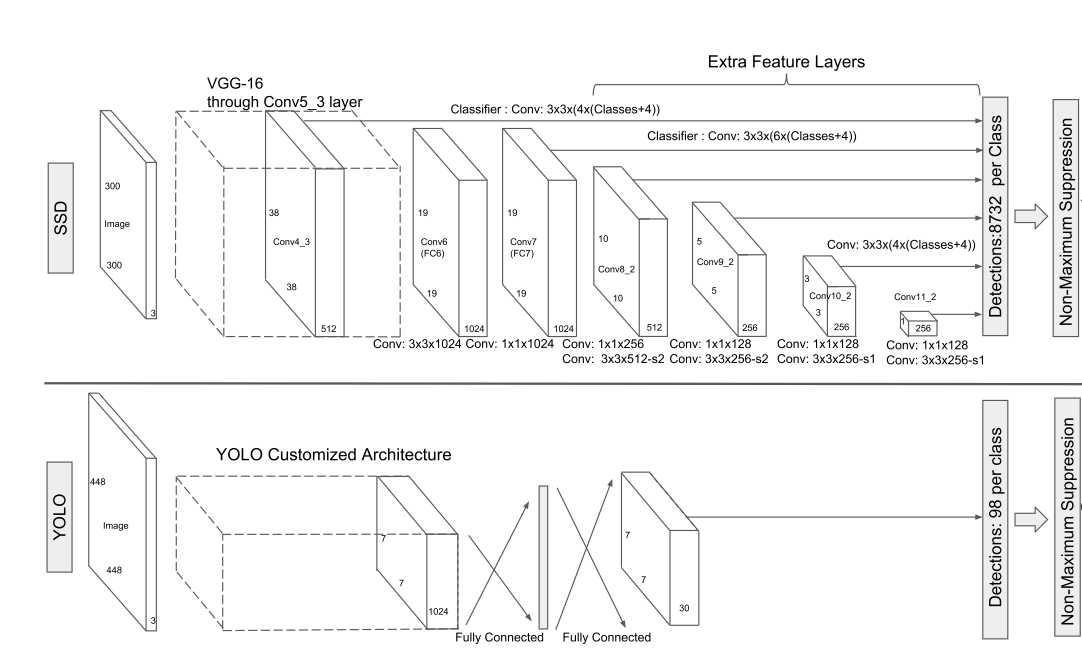
\includegraphics[height=2.5cm]{fig/architecture}
			\caption{Typical Architecture for One Stage Detectors}
			\label{fig:architecture}
		\end{minipage}
		\hspace{2cm}
		\begin{minipage}{0.4\textwidth}
			\centering
			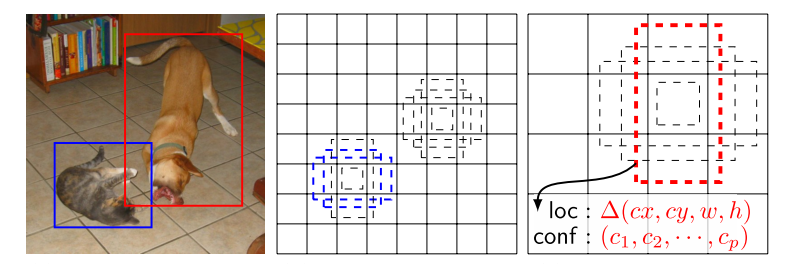
\includegraphics[height=2.5cm]{fig/anchors}
			\caption{Example of \cite{Liu}, the GT box of the cat is matched to two anchor boxes which get responsible for predicting that box. The GT box of the dog is matched to one anchor box.}
			\label{fig:anchors}
		\end{minipage}
	\end{figure}
	
	Most current methods rely on the same principle as Yolo/SSD: A convolutional regression layer is stacked on top of a "base network" that has been trained for image classification e.g. VGG-16. The output layer evaluates feature map(s) of the base network and predicts class confidences, and coordinate offsets for a predetermined set of bounding boxes (so called "prior boxes", "anchor boxes" or "default boxes"). The predictions are filtered in a final non-max-suppression step. During training one has to determine which anchor box is responsible for predicting a certain object. This "matching strategy" differs from method to method but is usually based on the intersection-over-union between the ground truth box and anchor box. \autoref{fig:anchors} illustrates the concept. The final loss function calculates the difference between the responsible boxes and the ground truth. 
	\todo{Elaborate}
	Within this framework several approaches exist that either change the base network or modify layers in between: \cite{ChengchengNing2017} propose to include an inception module in the network architecture to reduce computation while keeping/increasing performance. They also propose a more efficient non-max-suppression method. \cite{Wu} uses \textit{SqueezeNet} as base network and a mixture between the ssd and yolo loss function as training goal. \cite{Xiang} investigates the receptive fields of SSD and tries to incorporate more context, especially on lower feature maps, to increase detection rate for small objects.\cite{Linb} applies the framework for vehicle detection. They use \textit{GoogLeNet} as base network (and investigate several others).\cite{TripathiSanDiego} apply a network very similar to YoloV2 and investigate 8bit quantization of the model to make it runnable on embedded devices.
	
	A common problem of one stage detectors is the imbalance between background and object samples. Most methods upweigh the positive samples and/or use hard negative mining. \cite{Lin} introduces the \textit{Focal Loss} which focuses on sparse positive samples by design.
	

	
%	\subsection{\cite{Linb}}
%	
%	\begin{itemize}
%		\item Uses GoogLeNet as base network
%		\item investigates image augmentation and hard negative mining
%		\item Uses confidence score plus class probability although only one object shall be detected
%	\end{itemize}
%		
%	\subsubsection{YoloV3 \cite{Redmona}}
%	\begin{itemize}
%		\item binary cross entropy loss for class predictions
%		\item 3 boxes at each scale (3 scales)
%		\item merge lower level features with higher level features and predict another tensor
%		\item new network with several residual layers, in between 1x1 convolutions, fully connected layer at the end (53 layers)
%		\item runs at 22-51ms depending on resolution
%	\end{itemize}
%
%\begin{table}[]
%	
%	\caption{Object Detection}
%	\label{my-label}
%	\begin{tabular}{|p{3cm}|p{3cm}|p{3cm}|p{3cm}|p{3cm}|p{3cm}|p{3cm}|p{3cm}|}
%		\hline
%		& \multicolumn{3}{l|}{Traditional} & \multicolumn{4}{l|}{Deep}   \\ \hline
%		& Viola\&Jones    				   & HoG    & DPM   		   & R-CNN    & YOLO         & SSD & OverFeat \\ \hline
%		Feature Detector & Haar					   & HoG    & Multiple Hogs and virtual springs   & Learned by CNN     &  Learned by CNN            & & \\ \hline
%		Detection & \multicolumn{3}{l|}{Sliding Window, high filter responses indicate there is an object} & NN in sliding window detects regions for possible objects, For each proposed region a classification is run & Image is split in Grid each Grid spawns Bounding boxes and gives class probabilities & & \\
%		\hline
%		Accuracy (voc) &  & & & 73.2 mAP & 63.4 mAP & 74.3 mAP & \\ 
%		\hline
%		Speed & & & & 7 FPS (Faster-RCNN) & 45 FPS & 59 FPS & \\
%		\hline
%		Strengths & & & & & &  &\\
%		\hline
%		Weaknesses & & & & & &  &\\
%		\hline
%		\end{tabular}
%		
%		\end{table}



Each of the described group of methods has strengths and weaknesses. While shallow methods are typically quite fast they require a lot of manual effort and/or are not so accurate. Two-stage detectors on the other hand are quite accurate but their computational requirements are prohibitive for the hardware to be used in this thesis. One-stage detectors offer a compromise between detection accuracy and inference speed. In addition they can be trained end-to-end which requires only little manual engineering. However, the presented methods are still too slow for the hardware used in this thesis.


\todo{What do we define as wire frame object?}

\todo{Elaborate, It should become clear why we use deep learning}



\todoref{Wire detection}
\todoref{Method from last year, Other papers on drone racing}

\section{Hypothesis}

A small network should be able to learn the task.
\newpage
\section{Experiments}

\todo{Show how current methods perform on wire frame objects - performance over angle}
\todo{Reduce number of parameters and compare to big model}
\todo{What do the individual layers learn, where does it fail}

\section{Conclusion}